\documentclass[a4paper ,12pt, onecolumn]{article}
\usepackage[utf8]{inputenc}
\usepackage[spanish]{babel}
\usepackage[hidelinks]{hyperref}
\usepackage{graphicx}
\usepackage{hyperref}
\begin{document}
\title{Anexo desarrollo de hardware}

\author{Rubén Arce}
\date{\today}
\maketitle
\cleardoublepage
\tableofcontents
\listoffigures
\cleardoublepage

\section{Introducción}
    Los diseños eléctricos y trazado de las pistas del circuito se han llevado a cabo con Kicad en 
    su versión 5.1.6, se ha empleado este programa debido a que, en primer lugar es de software abierto y
    completamente gratuito y en segundo lugar debido a que corre en Linux y es capaz de llevar a cabo 
    cualquier diseño complejo sin problema.
    \paragraph{}
    Todas las PCBs se han llevado a cabo en dos capas con un espesor estándar de 1,6mm y con acabado superficial
    HASH plomo estaño en los primeros prototipos. En la verisión final se empleará acabado ENIG, o de oro 
    electrolítico para mejorar las especificaciones y durabilidad de la misma.

    Se han empleado tanto componentes SMD como through hole, se ha priorizado el precio en la selección de los mismos.
\section{Emisor beacon}
    \subsection{Aspectos a considerar}
        Las premisas para seleccionar el mejor microcontrolador han sido las siguientes: 
        \begin{enumerate}
            \item Bajo consumo
            \item Tamaño reducido
            \item Bluetooth y posibilidad de wifi en caso de eliminar el dispositivo emisor.
            \item Precio muy competitivo.
        \end{enumerate}
    \subsection{Circuito eléctrico}
        \subsubsection{Microcontrolador} 
            En el caso de microcontrolador se ha optado por un ESP32 de la empresa Espressif (\url{https://www.espressif.com/})
            debido en gran medida a que dispone de wifi y bluetooth así como de unas excelentes herramientas
            de desarrollo de software. 
        \subsubsection{Alimentación} 
            Para llevar a cabo la alimentación el microcontrolador y teniendo en cuenta que se han de garantizar los 3,3V en la entrada
            del micro se ha optado por una batería de Ion-Litio de 1400mAh que además tiene un tamaño reducido. El rango de tensión de la
            tarjeta va de 12V a 3,6V en el caso de que se opte por alimentarlo de otra forma.
    \subsection{PCB de control}
        \paragraph{}
        Una vez tenidas en cuenta estas especificaciones en el esquema eléctrico se ha llevado a cabo el ruteo de la tarjeta.
        \begin{center}
            \begin{figure}[ht]
                \centering
                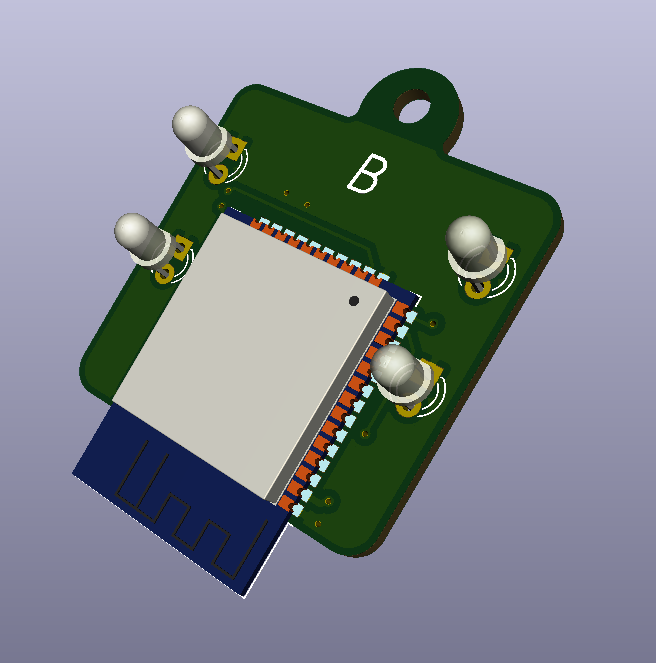
\includegraphics[width=0.4\textwidth]{../emiter_1.PNG}
                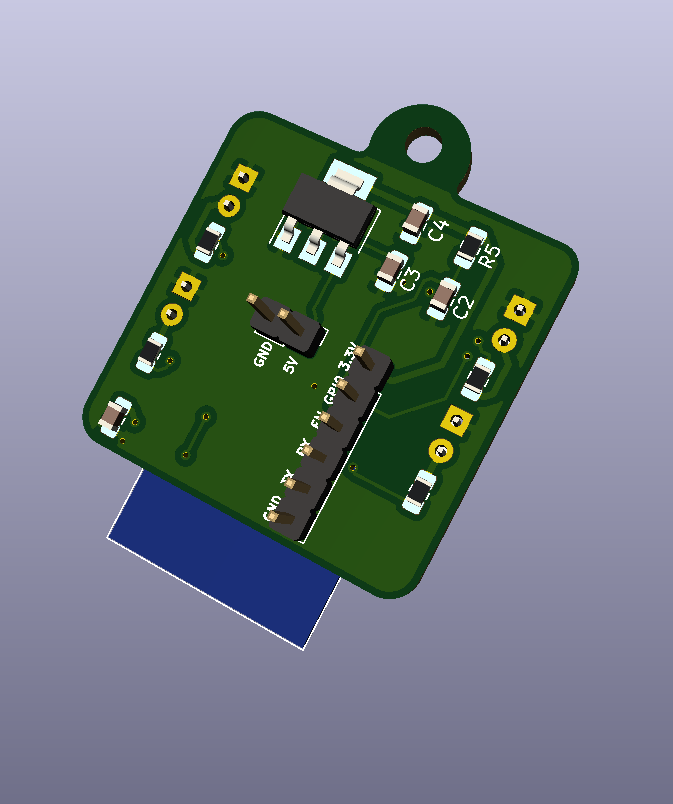
\includegraphics[width=0.35\textwidth]{../emiter_2.PNG}
                \caption{Renderizado de PCB del Beacon}
                \label{fig:mesh8}
            \end{figure}    
        \end{center}
        Vemos que se han llevado a cabo el trazado de pistas con planos de masa para evitar el efecto de la 
        electricidad estática de las personas no afecte demasiado a la electrónica.
        \begin{center}
            \begin{figure}[ht]
                \centering
                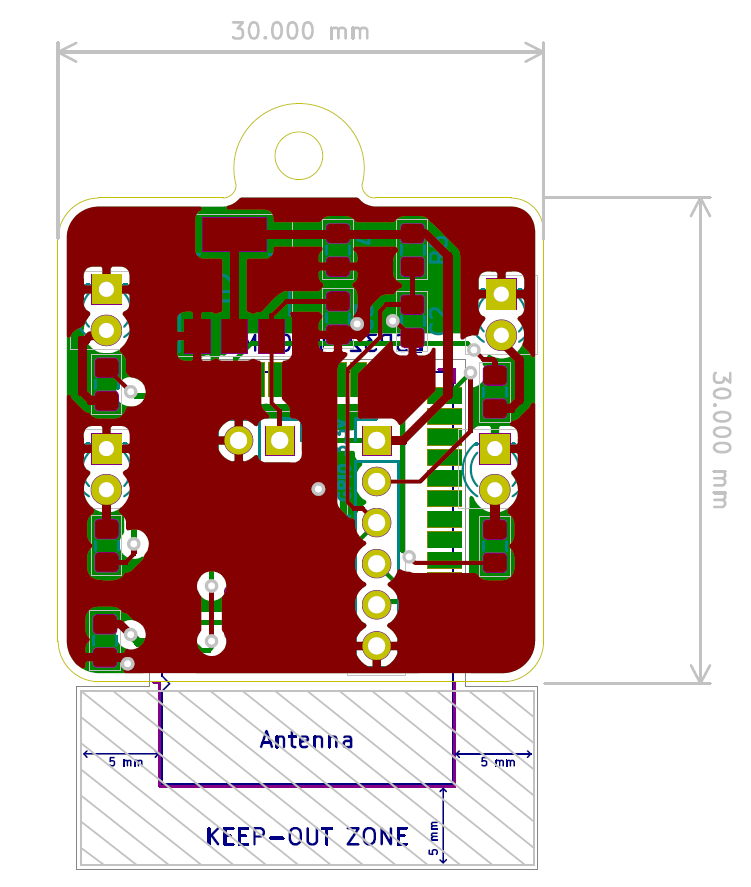
\includegraphics[width=0.40\textwidth]{../emiter_PCB.PNG}
                \caption{PCB del Beacon obtenida con Kicad}
                \label{fig:mesh9}
            \end{figure}    
        \end{center}
        Dejando lo más despejada la zona de la antena para mejor la ganancia de la misma y en conscuencia el alcance.
    \subsection{Imágenes reales}
        \paragraph{}
        Tras llevar a cabo la fabricación de las tarjetas prototipo estos son los resultados:
        \begin{center}
            \begin{figure}[ht]
                \centering
                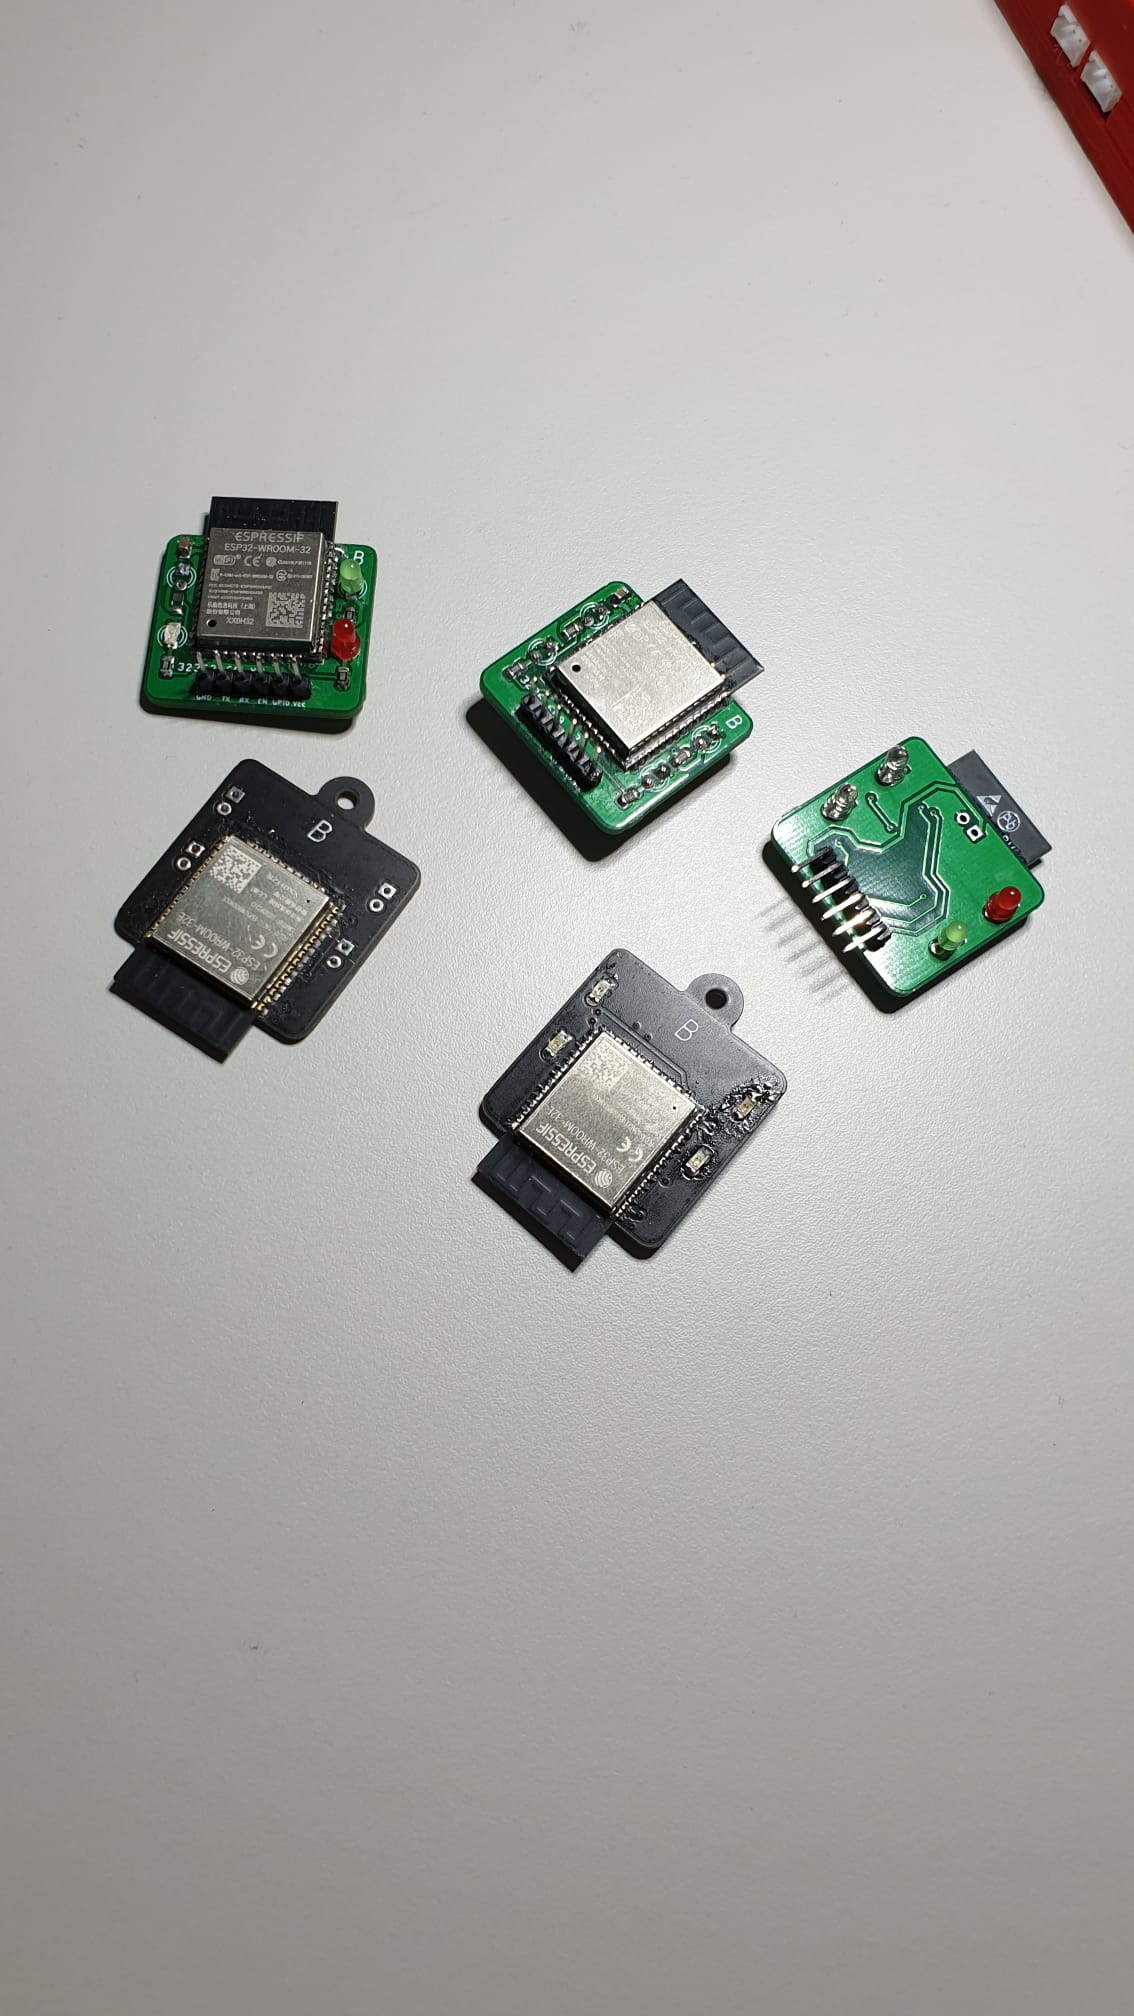
\includegraphics[width=0.5\textwidth]{../real_beacon_pcb.jpeg}
                \caption{Renderizado de PCB del master o gateway}
                \label{fig:mesh3}
            \end{figure}    
        \end{center}       
\section{Receptor beacon o gateway}
    \subsection{Aspectos a considerar}
        \begin{enumerate}
            \item Velocidad de procesamiento: el número máximo de equipos a localizar puede ser superior a 500, es por ello 
            por lo que quedan descartados los microcontrodores de 8bits y cristales de menos de 16MHz.
            \item Wifi/bluetooth: Han de escuchar a los beacons y subir los datos a internet, es por ello por lo que se hace 
            indispesable que cuente con los dos.
        \end{enumerate}

    \subsection{Circuito eléctrico}
        \subsubsection{Microcontrolador} 
            Teniendo en cuenta estas condiciones previas y contando con procesadores ESP32 del diseño anterior se ha optado por compartir 
            el procesador para ambos equipos. Con esto conseguimos que el software y librerías sean compatibles al 100\% y ahorre tiempo
            de desarrollo.
        \subsubsection{Alimentación} 
            En este caso y puesto que la tarjeta se encontrará estática en un lugar cercano a un enchufe se brindan las siguientes opciones
            de alimentación:
            \begin{enumerate}
                \item 220 VAC.
                \item 12 VDC.
                \item 5 VDC, en el caso de que se disponga de un ordenador cerca se podría conectar por USB.
            \end{enumerate}
            \begin{center}
                \begin{figure}[h]
                    \centering
                    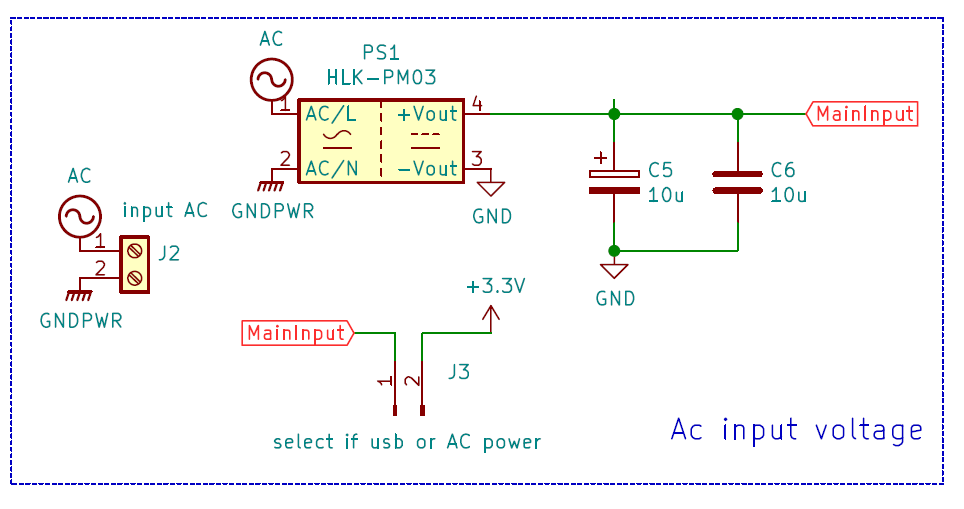
\includegraphics[width=0.8\textwidth]{../receiver_main_power.PNG}
                    \caption{Fuentes de alimentación de la PCB master}
                    \label{fig:mesh4}
                \end{figure}    
            \end{center}    
    \subsection{PCB de control}
        Se ha optado por llevar a cabo el trazado de pistas de alimentación por la cara top y por la bottom las de señal, vemos que hay dos 
        conectores en el extremos de la tarjeta, uno con una UART para comunicarse con otros sistemas de las planta y otro conector para sensores
        i2c, pensado para la lectura de humedad y temperatura y envío de estos datos a la web de control.
        \begin{center}
            \begin{figure}[ht]
                \centering
                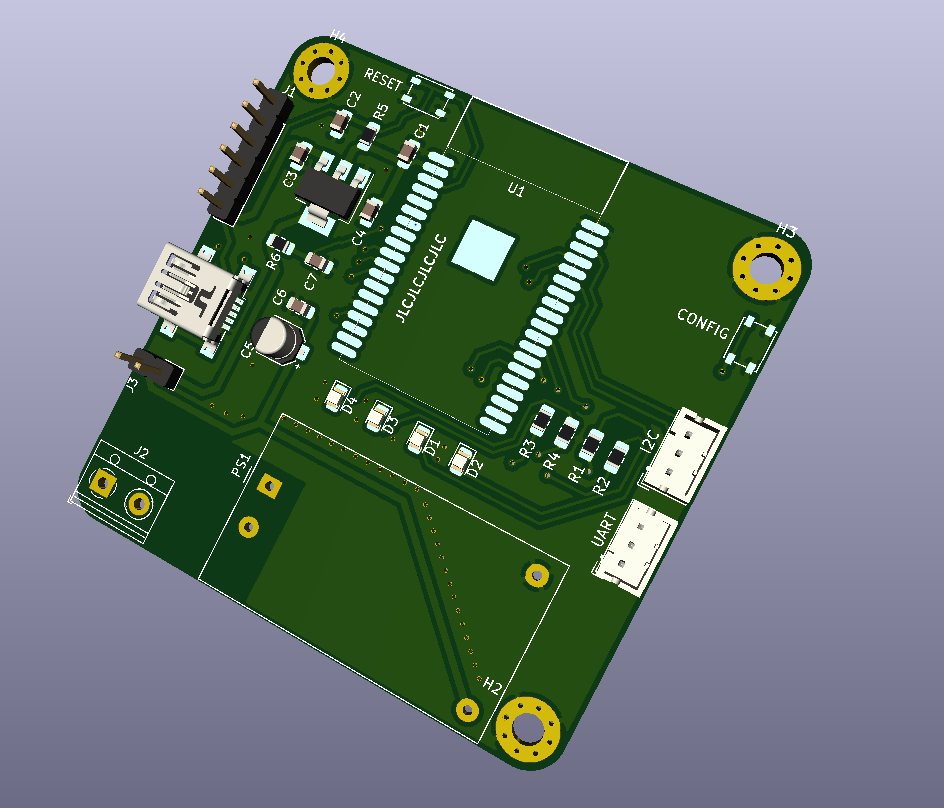
\includegraphics[width=0.4\textwidth]{../receiver_1.PNG}
                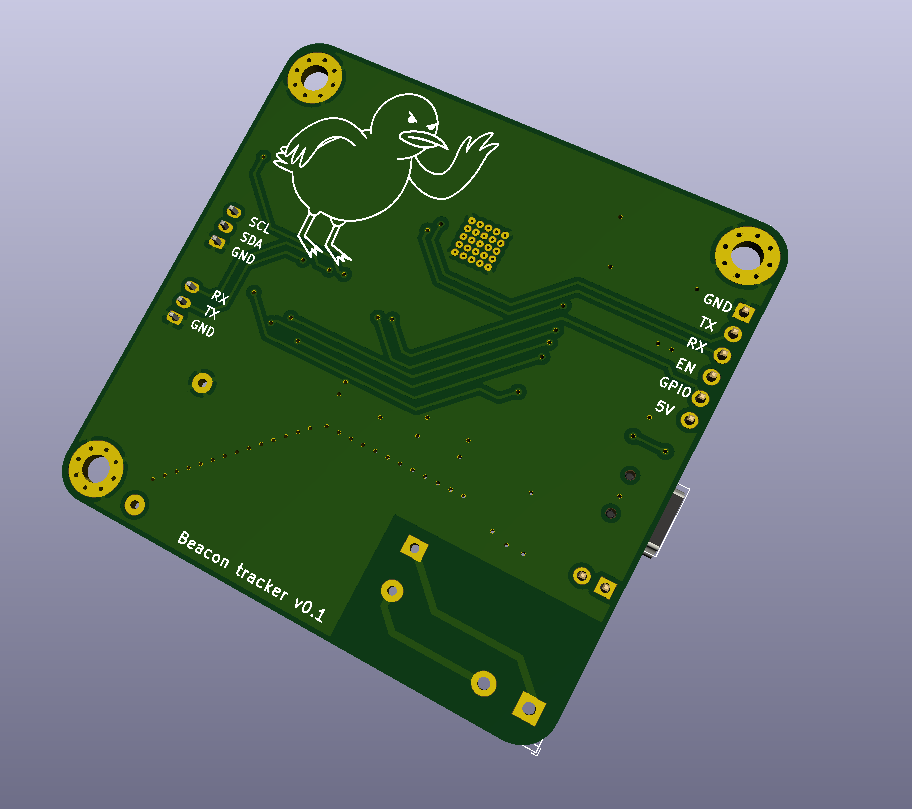
\includegraphics[width=0.4\textwidth]{../receiver_2.PNG}
                \caption{Renderizado de PCB del master o gateway}
                \label{fig:mesh5}
            \end{figure}    
        \end{center}
        En el apartado de planos se puede ver con mayor detalle el esquema eléctrico y dimensiones de la tarjeta.
        \begin{center}
            \begin{figure}[ht]
                \centering
                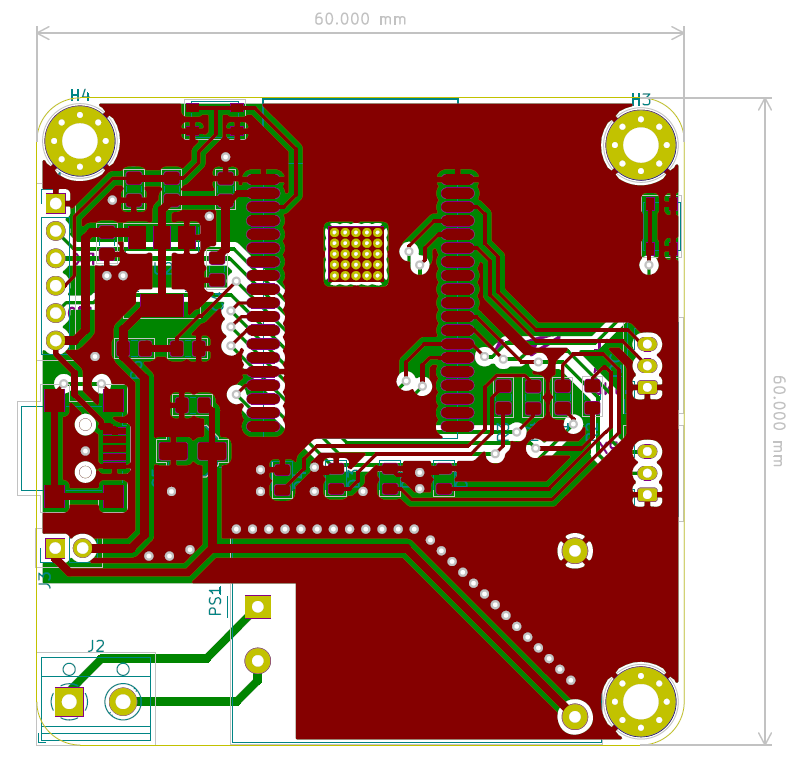
\includegraphics[width=0.5\textwidth]{../receiver_PCB.PNG}
                \caption{Renderizado de PCB del master o gateway}
                \label{fig:mesh6}
            \end{figure}    
        \end{center}
    \subsection{Imágenes reales}
        Por último y tras fabricar las tarjetas e imprimir las cajas que lo contienen se obtiene el siguiente resultado:
        \begin{center}
            \begin{figure}[ht]
                \centering
                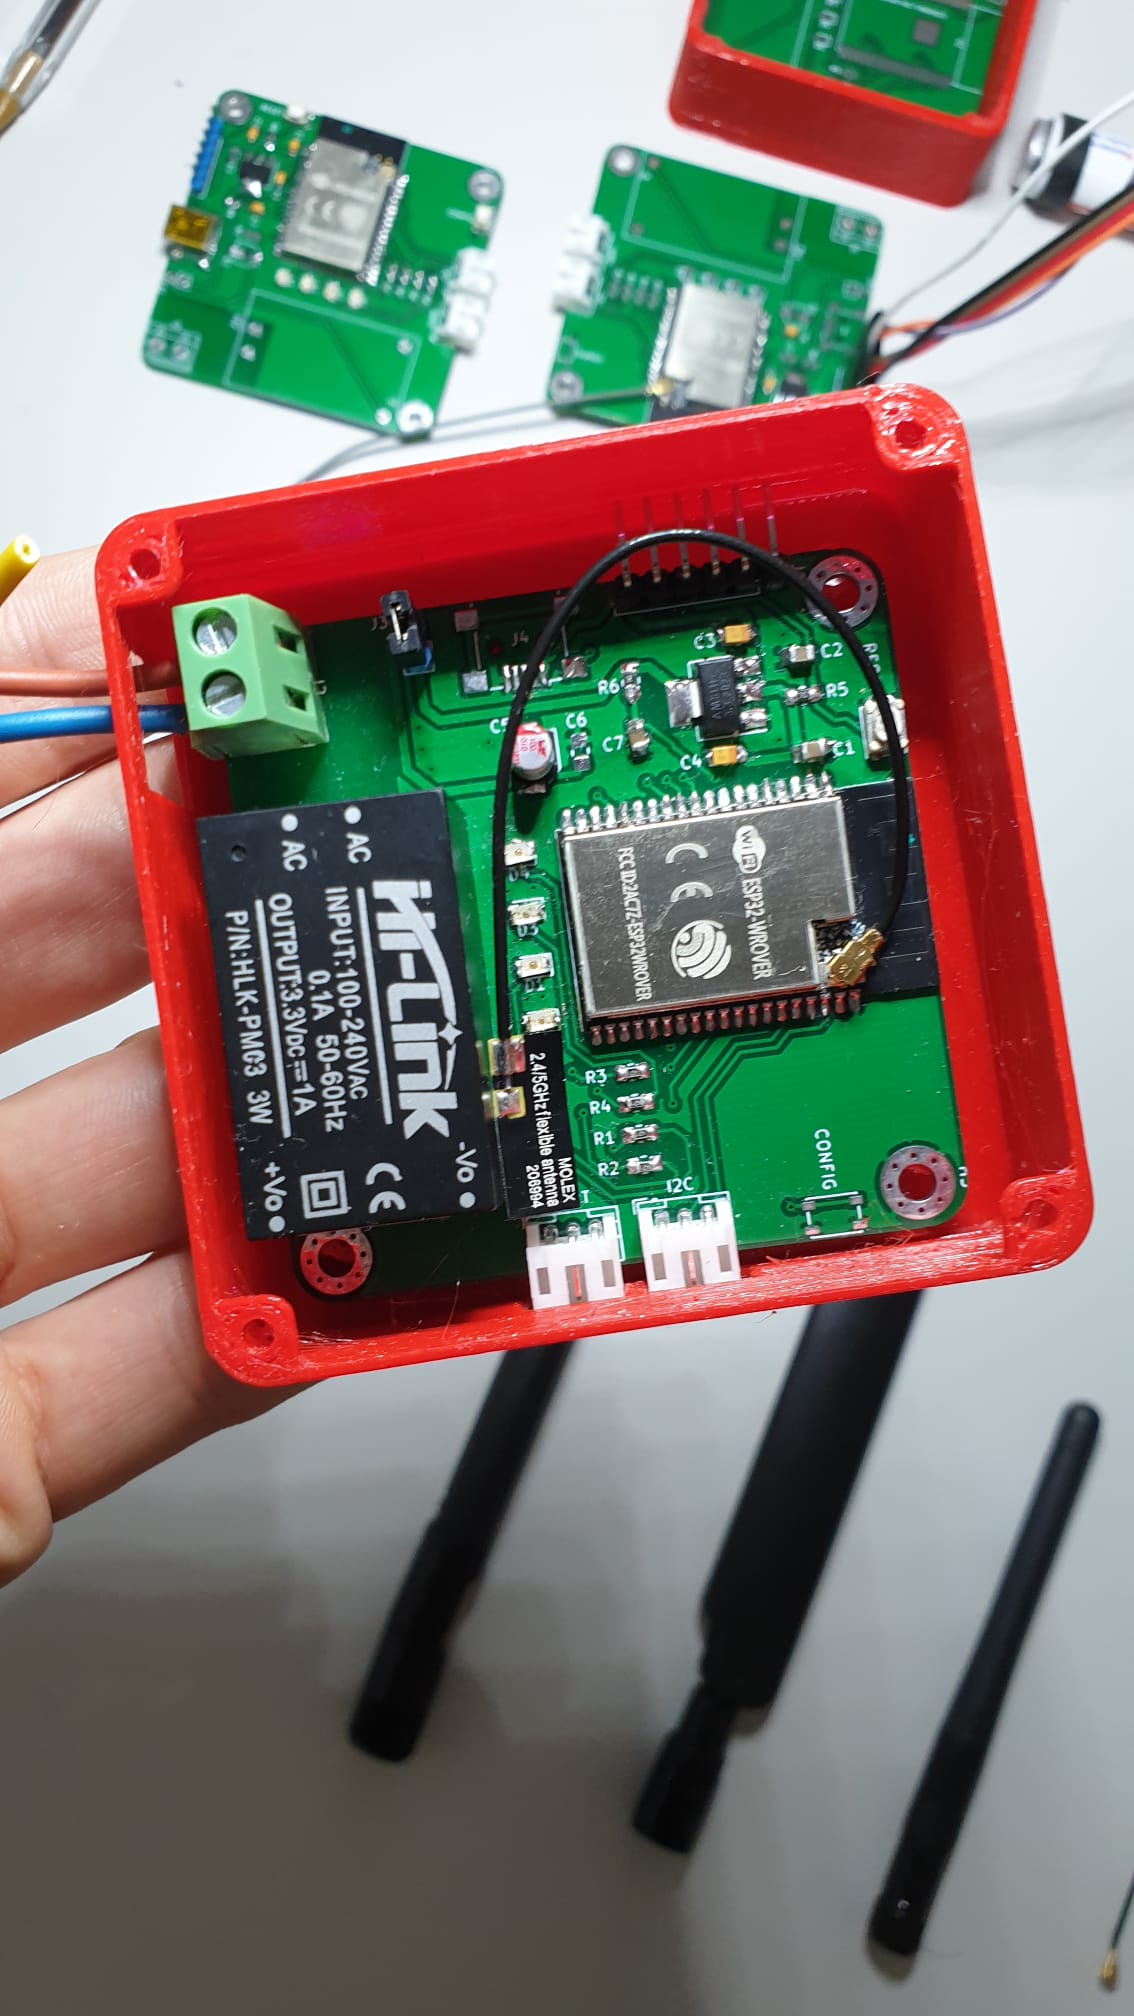
\includegraphics[width=0.4\textwidth]{../3d_antenna.jpeg}
                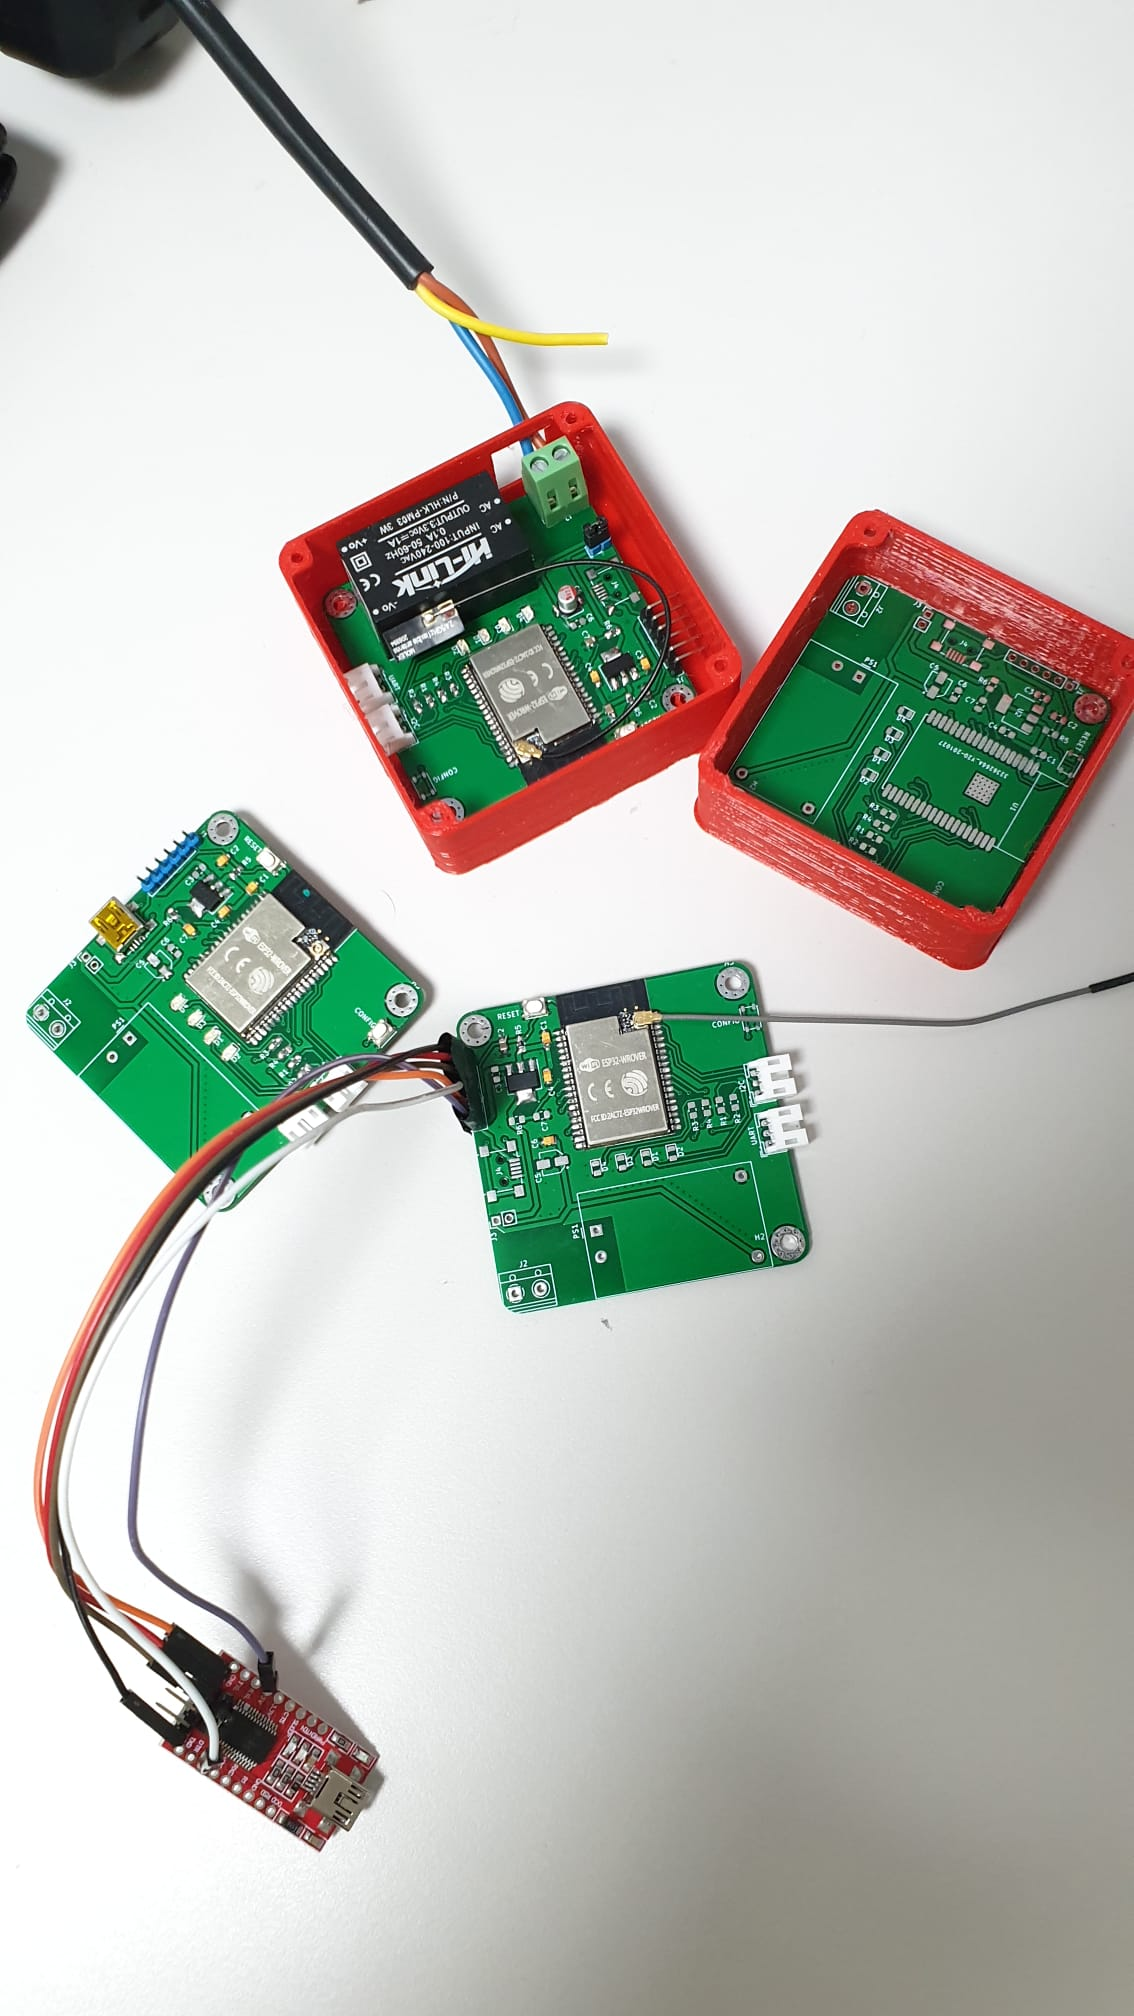
\includegraphics[width=0.51\textwidth]{../real_master_pcb.jpeg}
                \caption{Images reales de la PCB gateway}
                \label{fig:mesh7}
            \end{figure}    
        \end{center}
    \subsection{Conclusiones}
        Una vez recibidas las PCBs se fueron ensamblando y soldado a mano sin mayor incidentes que la confusión en la 
        posición de un led que por supuesto tras cargar el firmaware en la tarjeta no se iluminó.
        Solucionado el incidente y por suerte el versión 1 de las tarjetas fue la definitiva.
\end{document}